\chapter{Konttien orkestrointi\label{orchestration}}

Konttiteknologiaa käytetään kasvavissa määrissä monilla ohjelmistotuotannon osa-alueilla.
Konttiteknologia mahdollistaa fyysisen palvelimen tai ohjelmistökehittäjän tietokoneen suoritusympäristöstä eroavan vakaan ja rajattomasti toistettavan ympäristön \cite{Watada19}.
Konttiteknologian kasvava käyttö on luonut tarpeen hallinnoida suuria määriä kontteja samanaikaisesti.
Tähän tarpeeseen pyrkivät vastaamaan erilaiset konttiorkestraatioalustat.

Konttiorkestraatioalustat hallinnoivat suuria määriä kontteja jaetussa klusterissa.
Orkestraatioalustat, kuten Kubernetes, mahdollistavat muun muassa palveluiden replikoinnin, tehokkaan julkaisuketjun, kontitettujen palveluiden monitoroinnin ja virhetiloista toipumisen \cite{Khan17}.

\section{Kontti\label{container}}

% Maybe add something about container runtimes here?

Kontti on karsittu ympäristö, joka koostuu palvelusta ja sen tarvitsemista riippuvuuksista.
Kontti tarjoaa vakaan ja suljetun ympäristön palvelun suorittamiselle \cite{Watada19}.
Kontti on riippumaton fyysisestä palvelimesta ja sen ulkopuolisestä ympäristöstä, joka mahdollistaa saman kontin toistamisen muilla palvelimilla ja alustoilla \cite{Saha18}.

Virtuaalikonejulkaisuista poiketen useampi kontti voi jakaa resursseja ja näin ollen esimerkiksi käyttöjärjestelmän ydintä ei tarvitse säilöä erikseen jokaiseen konttiin.
Tämän seurauksena kontit ovat kokonsa ja käynnistysnopeutensa suhteen virtuaalikoneita tehokkaampi ratkaisu \cite{Dua14}.
Kuva~\ref{fig:container} esittää resurssien jaon eri julkaisuratkaisuilla.

Yleisesti käytettyjä konttiteknologiapalveluita ovat Docker ja Podman \cite{Abraham20, Bernstein14}.
Docker on suosittu ratkaisu, mutta vaatii toimiakseen aina käynnissä olevan palveluprosessin ja root-oikeudet palvelua suorittavaan käyttöjärjestelmään \cite{Abraham20}.
Nämä tekniset ongelmat ratkaisee esimerkiksi Podman, joka toimii ilman erillistä palveluprosessia ja root-oikeuksia \cite{Gantikow20}.
Konttien suoritysympäristöjä ovat muun muassa containerd ja CRI-O, joiden vaikutus palvelun suorituskykyyn on hyvin vähäinen \cite{torrez19, espe20}.

\begin{figure}[ht]
\begin{center}
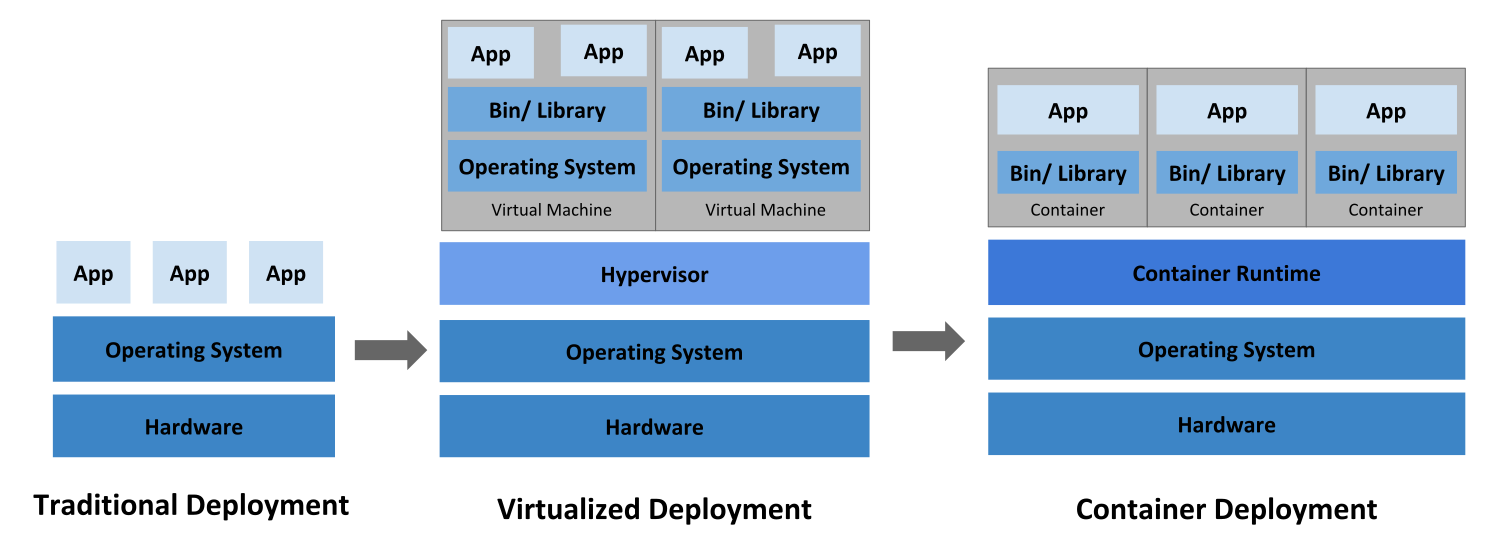
\includegraphics[width=0.9\textwidth]{figures/container_evolution.png}
\caption{Sovelluksen omat ja jaetut resurssit eri julkaisutavoilla \cite{Kubernetes23}\label{fig:container}.}
\end{center}
\end{figure}

\section{Konttiorkestraatioalustat\label{platforms}}

Erityisesti mikropalvelupohjaiset järjestelmät saattavat koostua useista sadoista konteista.
Myös muun muassa saman palvelun replikaatio ja alueellinen hajauttaminen luovat tarpeen hallinnoida suuria määriä kontteja \cite{Khan17}.
Konttiorkestraatioalustat ovat järjestelmiä, joiden tehtävä on mahdollistaa suurien konttimäärien hallinnointi.
Orkestraatioalustat muun muassa hallinnoivat konttien resurssien käyttöä, mahdollistavat konttien monitoroinnin ja huolehtivat konttien virhetilanteista toipumisesta \cite{Zhou21}.

Kubernetes on laajalti käytetty konttiorkestraatioratkaisu.
Se on nykyisistä ratkaisuista suorituskyvyltään tehokkain ja myös toiminnallisuuksiltaan kattavin \cite{Jawarneh19}.
Muita ratkaisuja ovat muun muassa Docker Swarm ja Amazon Elastic Container Service \cite{Khan17}.
Tässä tutkielmassa konttien orkestrointia käsitellään pääasiassa Kuberneteksen kautta.

Kubernetes on alkujaan Googlen kehittämä ja nykyään Linux Foundationin alla toimivan Cloud Native Foundationin hallinnoima avoimen lähdekoodin projekti \cite{Burns22}.
Kubernetes hallinnoi podeiksi kutsuttuja yhdestä tai useammasta kontista koostuvia kokonaisuuksia.
Kubernetes-klusteri muodostuu useista fyysisistä palvelimista tai virtuaalikoneista, joita kutsutaan nodeiksi \cite{Medel18}.
Kubernetes mahdollistaa muun muassa seuraavat asiat \cite{Zhou21}:

\begin{itemize}
\item Resurssien käyttörajojen hallinta (engl. \textit{resource limit control}): Muisti- ja suoritinresurssien minimi- ja maksimimäärän asettamisen konttikohtaisesti.
\item Vuoronvalvonta (engl. \textit{scheduling}): Konttien automaattinen ja optimoitu sijoitus eri nodejen välillä.
\item Kuormituksen tasaaminen (engl. \textit{load balancing}): Kuormituksen jakaminen useiden konttien välillä. 
\item Terveystarkastus (engl. \textit{health check}): Konttien toimivuuden tarkastus ja viallisiin kontteihin reagointi.
\item Vikasietoisuus (engl. \textit{fault tolerance}): Automaattinen uusien konttien luonti ja viallisten tuhoaminen virhetilanteissa.
\item Automaattinen skaalautuminen (engl. \textit{auto-scaling}): Konttien lisääminen tai poistaminen automaattisesti kuormituksen mukaan.
\end{itemize}

Kuva \ref{fig:kubernetes} esittää Kuberneteksen eri komponentit. Kubernetes-klusteri koostuu useasta podeja suorittavista nodeista.
Koko klusteria hallinnoi \textit{Control Plane}, joka sisältää klusterin hallinnointiin käytetyn REST-rajapinnan, podien jakautumisesta nodejen välillä huolehtivan vuorontajan sekä pysyväistallennetun avainarvosäilön.
Näiden lisäksi \textit{Control Plane} sisältää useita \textit{Controller manager}-prosesseja, jotka hallinnoivat eri resursseja.
Erityisesti \textit{Cloud controller manager} on komponentti, joka mahdollistaa Kubernetes-klusterin yhdistämisen eri pilvialustojen rajapintojen kanssa \cite{components23}.

\begin{figure}[ht]
\begin{center}
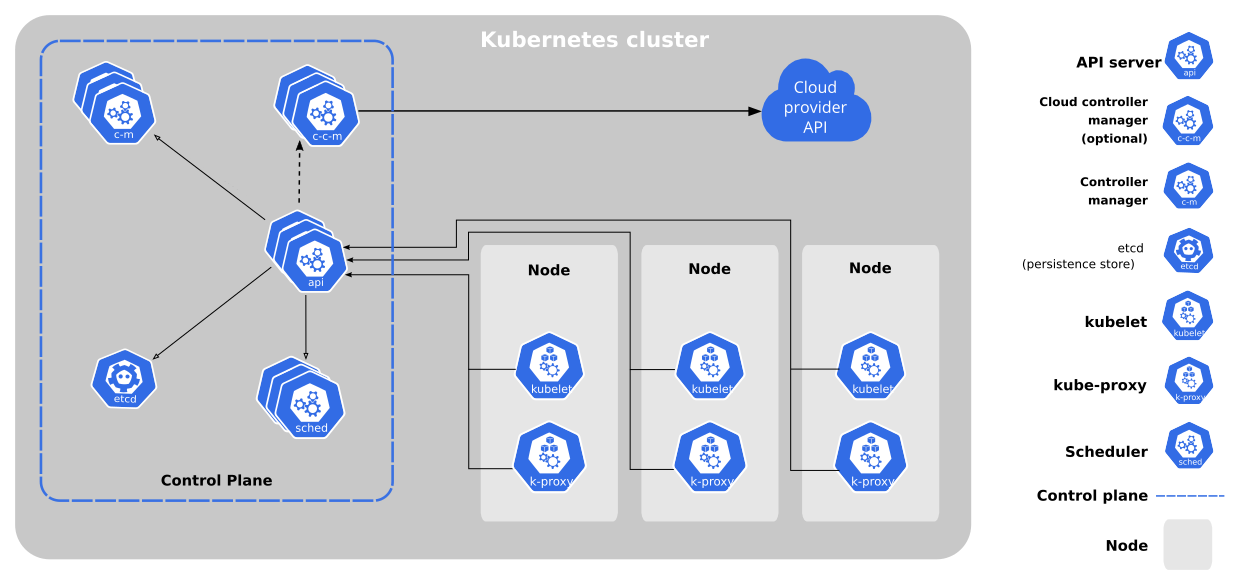
\includegraphics[width=1\textwidth]{figures/kubernetes_components.png}
\caption{Kuberneteksen komponentit \cite{components23}\label{fig:kubernetes}.}
\end{center}
\end{figure}

\section{Konttien orkestrointi ja DevOps-toimintamalli\label{orchestration:devops}}

Konttiteknologiaa ja konttien orkestrointia käytetään usein osana DevOps-toimintamalliin perustuvaa ohjelmistotuotantoa \cite{Kang16, Narasimhulu23}.
Konttiteknologia avulla samaa kontitettua palvelua voi siirtää eri ympäristöjen välillä.
Konttiteknologia mahdollistaa myös koko palvelun ympäristön konfiguroinnin ja näin ennustettavamman toiminnan ja helpomman vianmäärityksen \cite{Narasimhulu23}.

Kontin siirrettävyys mahdollistaa tehokkaan varmennus- sekä julkaisuvaiheen DevOps-toimintamallissa, koska samaa konttia voidaan ensin käyttää testauksessa ja sen jälkeen siirtä se esimerkiksi julkaisualustana toimivalle konttiorkestraatioalustalle.
Kontin ympäristön konfiguroitavuus taas auttaa operointi- ja monitorointivaiheissa.
Kontin erikseen määritettävästä ympäristöstä voi olla hyötyä myös kehitysvaiheessa, koska se mahdollistaa useille kehittäjille samanlaisen tuotantoympäristöä muistuttavan kehitysympäristön.

Luvussa \ref{platforms} käsitellyt Kuberneteksen tarjoamat konttien orkestrointipalvelut tukevat myös hyvin DevOps-toimintamallia.
Resurssien käytön hallinta, aikataulutus, kuormituksen tasapainottaminen ja automaattinen skaalautuminen tukevat kaikki hyvin operointivaihetta.
Terveystarkastus ja vikasietoisuus taas tukevat monitorointia.
Konttiorkestraatioalustan käyttö myös itsessään mahdollistaa konttiteknologian käytön palvelun julkaisuratkaisuna, joka tekee saman kontin käytöstä testauksessa ja tuotantokäytössä mahdollista.

% Maybe show an example of a DevOps based Container orchestration flow

Konttiteknologian ja konttien orkestroinnin käytöstä osana DevOps-toimintamallia on löytynyt paljon etuja.
Seuraavaksi tarkoituksena on tarkastella muita julkaisutapoja ja niiden soveltuvuutta DevOps-toimintamallin mukaiseen ohjelmistotuotantoon.
Näitä julkaisutapoja verrataan myös konttiteknologian ja konttien orkestraation käyttöön.
